% !TeX root = ../tg.tex

\chapter{低质量数据下分割联邦学习的性能优化}
\section{基于分割-联邦学习的鲁棒性算法}
为了解决 SFL 中的标签噪声问题，我们在 SFL-V2 的基础上提出了 SF-LCT 算法。SF-LCT 受文献 \cite{b9} 中一种应对联邦学习（FL）中标签噪声算法FedCorr的启发。与已有工作不同的是，我们联合处理了分割-联邦学习中的非独立同分布（non-IID）数据和标签噪声问题，通过利用分割-联邦学习中服务器端可用的标签信息，并结合基于熵的思想来进行噪声检测。

为了评估 SF-LCT 在实际场景中的性能，我们搭建了一个实验测试平台来实现该算法，这需要精心设计（例如并行传输、高效的内存与 CPU 使用），以减少训练延迟。接下来，我们将首先介绍算法的具体细节,然后介绍实验测试平台的设计。
\subsection{算法设计}
\begin{algorithm}[t]
\caption{SF-LCT 算法}\label{alg1}
\begin{algorithmic}[1]
\STATE 初始化全局模型 $\omegab=(\omegabc,\omegabs)$ 和本地模型 $(\omegab_n, n\in\N)$，其中 $\omegab_n = (\omegabcn, \omegabs)$；
\STATE \underline{// \textit{第一阶段：噪声检测}}
% \STATE $avg(d)\leftarrow \sum_{n\in\N} d_n$
\STATE 根据 \eqref{calculate dn} 计算每个客户端 $n$ 的系数 $\gamma_n$；
\IF{$\max_{n\in \mathcal{N}} \{\gamma_n\} > \tau$}
\STATE 根据 \eqref{eq:LE} 计算每个客户端 $n$ 的 $\text{LE}_n$；
\STATE 基于所有 $n\in\N$ 的 $\text{LE}_{n}$，使用高斯混合模型（GMM）识别出干净客户端集合 $\N_{cle}$ 与含噪客户端集合 $\N_{noi}$；
\ELSE
\STATE $\omegab\leftarrow$ 所有客户端使用其数据集 $\mathcal{D}_n$，按照第 \ref{subsec:training} 节中步骤 1--4 进行 $R_0$ 轮 SFL 训练；
\STATE 根据 \eqref{definition of lid} 计算每个客户端 $n$ 的 $\text{LID}_n$；
\STATE 基于所有 $n\in\N$ 的 $\text{LID}_{n}$，使用 GMM 识别出干净客户端集合 $\N_{cle}$ 与含噪客户端集合 $\N_{noi}$；
\ENDIF
\STATE $\omegab\leftarrow$ 所有客户端 $n\in\N$ 使用其数据集 $\mathcal{D}_n$，按照第 \ref{subsec:training} 节中步骤 1--4 继续进行 SFL 训练，直到完成 $R_1$ 轮；
\STATE \underline{// \textit{第二阶段：噪声修正}}
\STATE $\omegab\leftarrow$ 干净客户端集合 $\mathcal{N}_{cle}$ 使用其数据集 $\mathcal{D}_n$，按照第 \ref{subsec:training} 节中步骤 1--4 进行 $R_2$ 轮 SFL 训练；
\STATE $loss_{n,i} \leftarrow$ 每个客户端 $n$ 中每条数据 $i$ 的测试损失；
\FOR{每个客户端 $n \in \N_{noi}$}
\STATE $\Dnoih_n\leftarrow$ 对所有 $i$ 上的 $loss_{n,i}$ 使用 GMM 进行分类，识别出含噪数据集合；
\FOR{每个 $(x_i,\tilde{y}_i)\in\Dnoih_n$}
\STATE 客户端 $n$ 计算 $h(x_i;\omegabcn)$ 并将 smashed data 发送给训练服务器；
\STATE 训练服务器计算 $h(x_i;\omegab_n)$，并基于输出 $h\left(x_i;\omegab_n \right)$ 修正标签 $\tilde{y}_i$；
\ENDFOR
\ENDFOR
\STATE \underline{// \textit{第三阶段：SFL 训练}}
\STATE $\omegab\leftarrow$ 所有客户端 $n\in\mathcal{N}$ 使用更新后的数据集 $\mathcal{D}_n'$（已完成标签噪声修正）按照第 \ref{subsec:training} 节中步骤 1--4 进行 $R_3$ 轮 SFL 训练；
\RETURN $\omegab$.
\end{algorithmic}
\end{algorithm}

SF-LCT 的核心思想是先检测再修正标签噪声。该算法包含三个阶段：

 \textbf{第一阶段：} 使用本地内在维度（LID）检测独立同分布数据中的含噪客户端，使用标签熵（LE）检测非独立同分布数据中的含噪客户端。
 \textbf{第二阶段：} 利用来自干净客户端的数据训练全局模型，然后检测并修正来自含噪客户端的错误标签。
 \textbf{第三阶段：} 在修正后的数据样本上进行传统的 SFL 训练。

为便于表述，我们使用 $\omegab$ 表示需要训练的全局模型，并省略训练轮次的索引。需要注意的是，每个阶段（特别是第二或第三阶段）所使用的初始全局模型是前一阶段训练完成的模型。我们用 $\D_{n}$ 表示客户端 $n$ 的原始数据集。在第二阶段中，部分含噪标签会被修正，从而得到客户端 $n$ 的更新数据集，记作 $\D_{n}'$。

SF-LCT 算法的伪代码如 算法~\ref{alg1} 所示，图~\ref{fig:SF-LCT} 展示了 SF-LCT 的整体流程。

\begin{figure}[t]
\centering
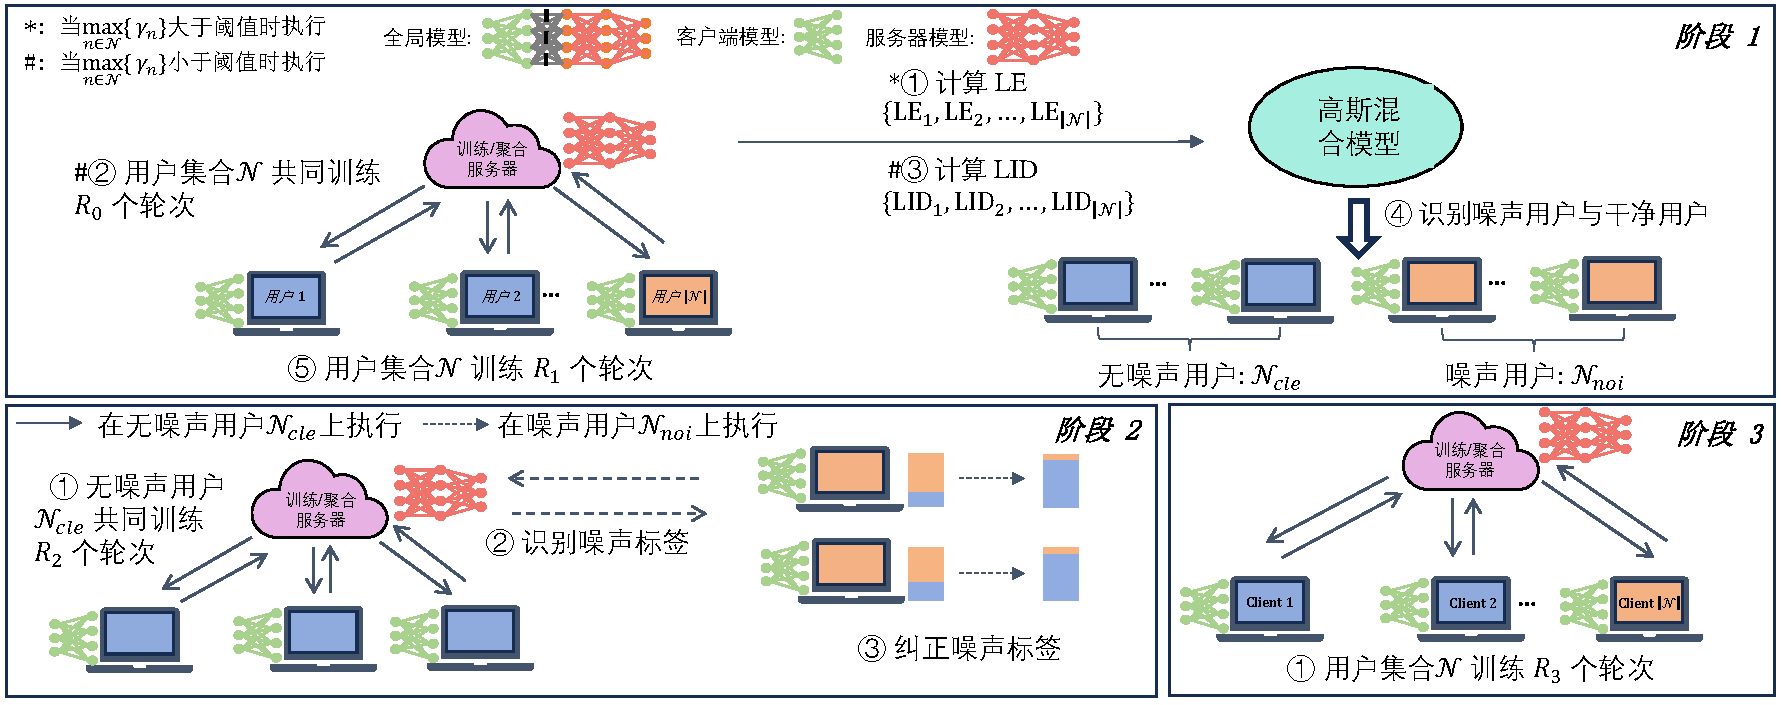
\includegraphics[width=\linewidth]{figures/al.pdf}
\caption{SF-LCT 概览。}
\label{fig:SF-LCT}
\end{figure}

\begin{figure}[t]
\centering
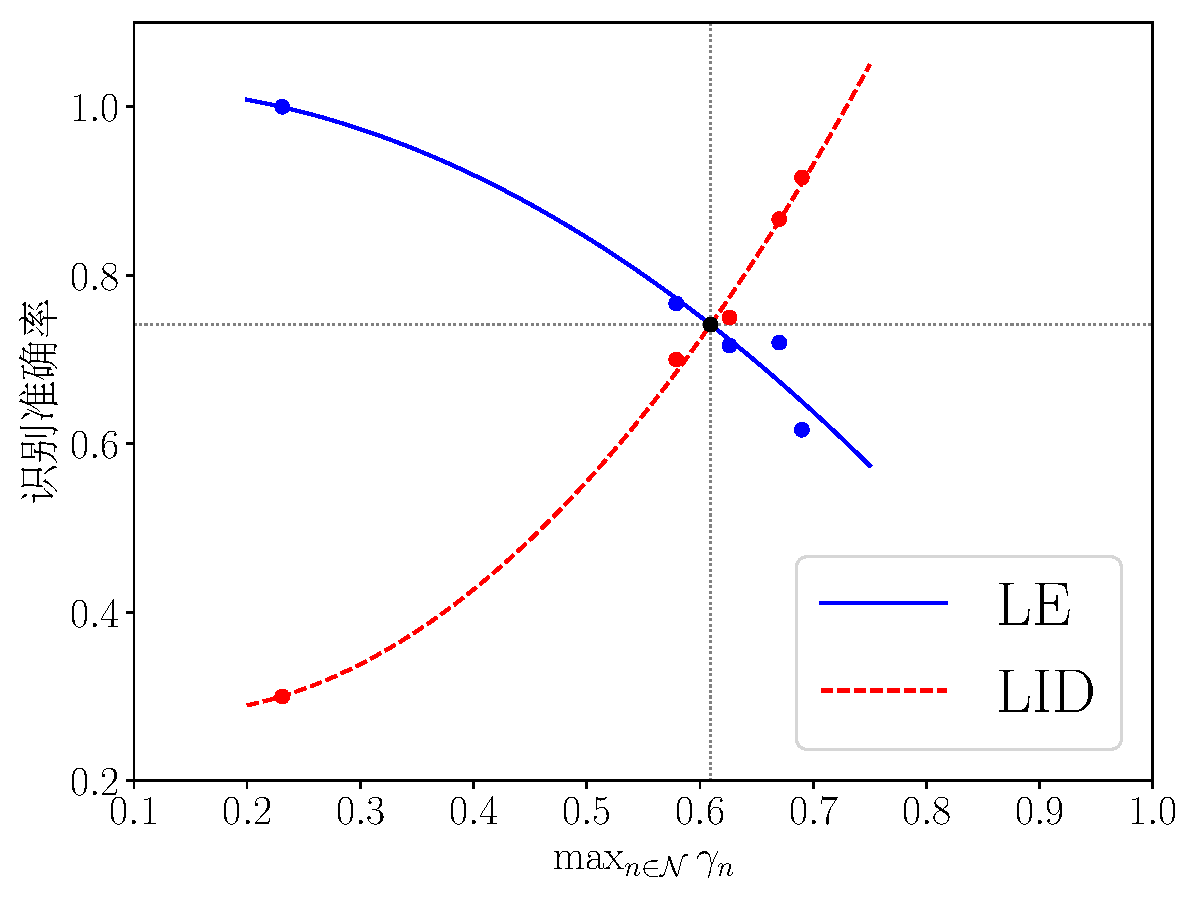
\includegraphics[height=5.3cm]{figures/gamma.pdf}
\caption{通过 LE 和 LID 方法检测含噪用户的准确率与 $\max_{n\in \mathcal{N}} \gamma_n$ 的关系。}
\label{fig:gamma}
\end{figure}

第一阶段的目标是检测存在标签噪声的客户端。在分割-联邦学习中，客户端会在训练过程中将标签发送给服务器 \cite{thapa2022splitfed,huang2023minibatch}。服务器为每个客户端 $n$ 计算一个系数 $\gamma_n$，用以反映该客户端数据集的非独立同分布（non-IID）程度。

为了计算 $\gamma_n$，服务器按升序排列客户端 $n$ 的标签频率。设 $(y_{(1)}^n, y_{(2)}^n, \dots, y_{(|\mathcal{K}|)}^n)$ 表示排序后的标签。

然后，$\gamma_n$ 通过计算前 $\lfloor K/{2}\rfloor$ 个标签所占数据样本的比例来确定：
\begin{equation}\label{calculate dn}
\gamma_n = \frac{\sum_{i=1}^{\lfloor K/{2}\rfloor} \text{count}(y_{(i)}^n)}{|\D_n|},
\end{equation}
其中 $\text{count}(y_{(i)}^n)$ 表示具有标签 $y_{(i)}^n$ 的数据样本数量。

根据所有 $n\in\N$ 的 $\gamma_n$ 值，我们选择合适的方法来检测含噪客户端。有两种候选方法：基于 LID 的检测和基于 LE 的检测。前者来源于文献 \cite{b9}，更适合 IID 数据集场景；后者则更适用于 non-IID 数据集。我们建议使用 $\max_{n\in \mathcal{N}} \gamma_n$ 来判断是否存在数据集极度非 IID 的客户端（即仅包含有限种类的标签）。如果 $\max_{n \in \mathcal{N}} \gamma_n > \tau$，则优先采用基于 LE 的方法；否则推荐使用基于 LID 的方法。其中，$\tau$ 是一个可以通过实验经验确定的阈值。

以 CIFAR-10 数据集为例，图~\ref{fig:gamma} 中的两条曲线展示了在不同 $\max_{n \in \mathcal{N}} \gamma_n$ 值下，LE 和 LID 方法检测含噪客户端的准确率。这两条曲线的交点表示最优的 $\tau$ 值，在该点上两种方法的性能达到平衡。对于这两种方法，训练服务器会通过计算每个客户端的 LID 分数或 LE 分数来评估其是否含有标签噪声。

\textbf{LID 分数：} 为了计算客户端的 LID 分数，首先让客户端使用 SFL 对全局模型进行 $R_0$ 轮训练。根据训练输出，对每个数据点 $(x_i,\tilde{y}_i)$，其 LID 定义如下 \cite{b9,amsaleg2015estimating,houle2013dimensionality}：
\begin{align}\label{eq:lid}
\text{LID}(x_i,\tilde{y}_i)=-\left(\frac{1}{k}\sum_{j=1}^k\log\frac{d_j\left(h\left(x_i,\omegab\right)\right)}{d_{max}\left(h\left(x_i,\omegab\right)\right)}\right)^{-1}.
\end{align}
在式 \eqref{eq:lid} 中，$d_j\left(h\left(x_i,\omegab\right)\right)$ 表示数据样本 $(x_i,\tilde{y}_i)$ 与其邻近样本 $(x_j,\tilde{y}_j)$ 在特征空间中的欧氏距离。考虑 $(x_i,\tilde{y}_i)$ 的 $k$ 个最近邻样本，即 $k$ 个具有最小 $d_j\left(h\left(x_i,\omegab\right)\right)$ 的样本。令 $d_{max}\left(h\left(x_i,\omegab\right)\right)$ 表示在这 $k$ 个最近邻中与 $(x_j,\tilde{y}_j)$ 的最大距离。

直观上讲，定义在 \eqref{eq:lid} 中的数据样本 LID 反映了该样本与其他样本的接近程度，从而间接揭示了其标签可能为噪声标签的可能性。每个客户端 $n$ 的 LID 分数为其数据集 $\mathcal{D}_n$ 中所有样本 LID 值的平均值：

\begin{equation}\label{definition of lid}
\textstyle \text{LID}_n = \sum_{(x_i,\tilde{y}_i)\in\D_{n}} \text{LID}(x_i,\tilde{y}_i)/|\D_n|.
\end{equation}

\textbf{LE 分数：} 我们提出使用标签的熵来衡量标签噪声。这一想法源于一个直观认识：随机噪声会使标签分布变得不那么集中。具体而言，LE 分数的计算方式如下：
\begin{equation}\label{eq:LE}
\text{LE}_n=-\gamma_n\log(\gamma_n)-(1-\gamma_n)\log(1-\gamma_n).
\end{equation}

随后，SF-LCT 使用高斯混合模型（GMM）对 LID 或 LE 分数进行分类，从而区分干净客户端与含噪客户端。接着，SFL 训练过程继续进行，直到完成 $R_1$ 轮训练。需要注意的是，LID 的计算需要 $R_0$ 轮训练，而 LE 则不需要。进行至 $R_1$ 轮的训练确保了基于 LID 和基于 LE 的方法在相同训练水平上进行比较。

第二阶段通过使用被归类为干净的客户端（即 $n \in \mathcal{N}_{cle}$）来训练全局模型 $\omegab$，以提升模型准确率。训练损失用于识别每个含噪客户端 $n\in\mathcal{N}_{noi}$ 数据集中的噪声标签，因为噪声数据的损失通常较高。训练好的模型 $\omegab$ 随后被用于修正刚刚检测出的噪声标签。

在第三阶段，所有客户端 $n \in \mathcal{N}$ 在已修正第二阶段中检测出的噪声标签的数据集 $\mathcal{D}_n'$ 上继续进行训练，共进行 $R_3$ 轮。最终，获得优化后的全局模型。

\subsection{树莓派测试平台的实现}\label{sec:testbed}
\begin{figure}[htbp]
\centering
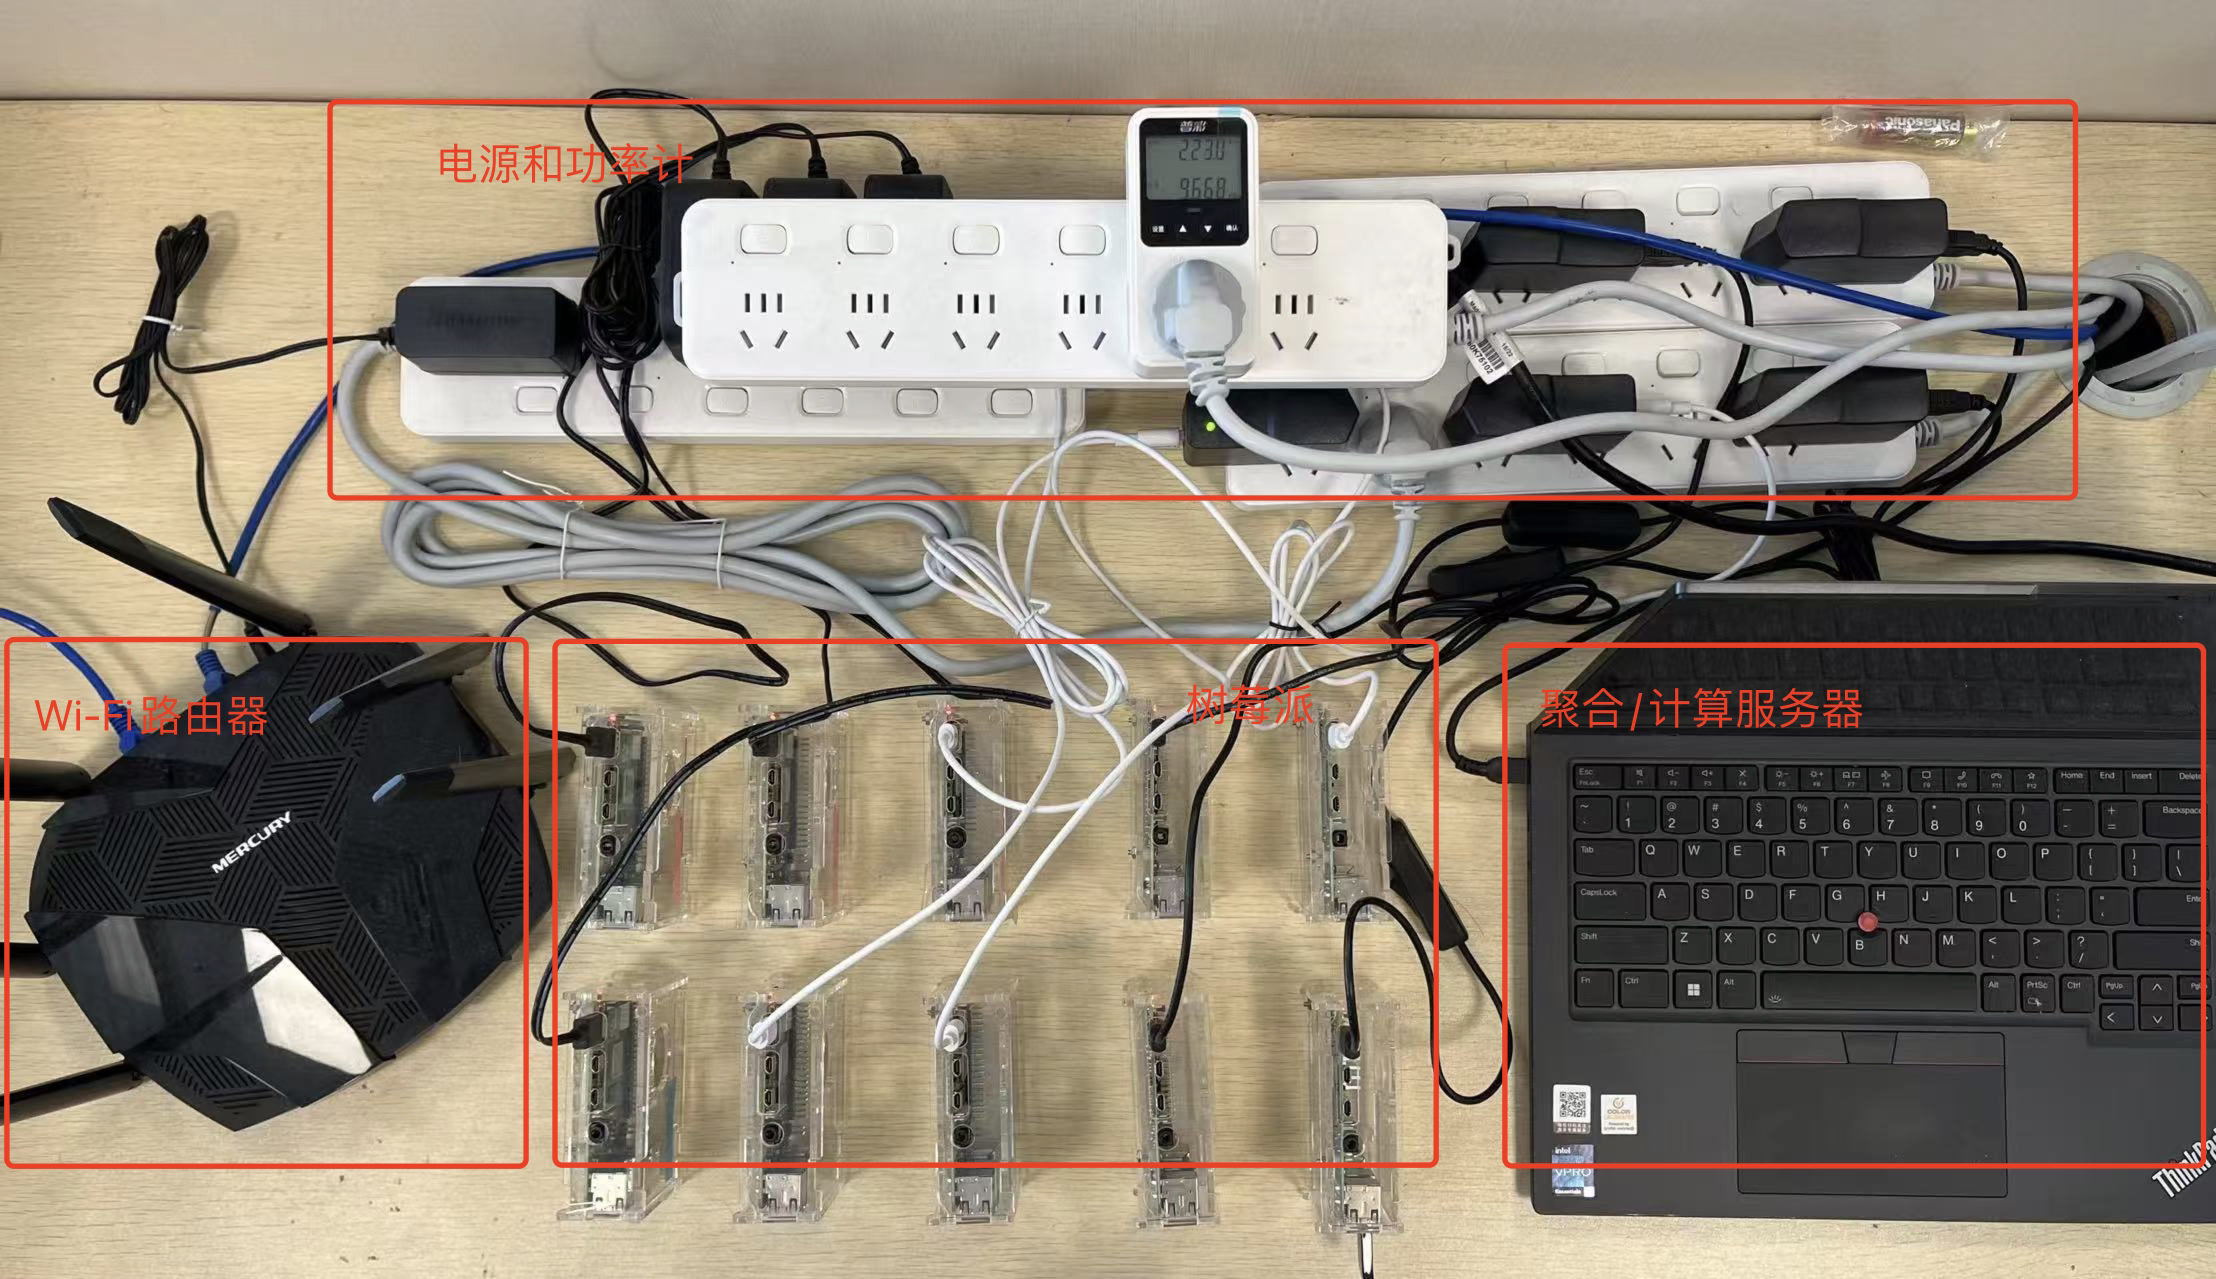
\includegraphics[height=4.5cm]{figures/testbed.png}
% \vspace{-5pt}
\caption{真实测试平台}
\label{fig:testbed}
% \vspace{-15pt}
\end{figure}
为了测试SF-LCT在真实世界中的能耗情况,本文使用树莓派和个人电脑搭建了测试平台，用来测试SF-LCT与其他各种基准算法的能耗比较。如图~\ref{fig:demo}所示，我们的测试平台主要分为两个模块：客户端和服务器，其中服务器包括训练服务器和联邦服务器。每一个客户端都拥有一个HTTP服务器和HTTP下载器，
用于向服务器提供中间激活值和从下载中间梯度；类似的，服务器上也有$N$个HTTP服务器和一个HTTP下载器，用于向客户端提供中间梯度和下载中间激活值，其中每一个HTTP服务器都与一个客户端严格对应。我们设计的测试平台支持并行数据交换，使用HTTP协议传输
数据可以消除因网络信号导致的信息损失。并且服务器HTTP服务器与客户端一一对应的设计可以避免网络情况较差的情况下出现传输中断。

如图~\ref{fig:testbed}所示，我们真实的测试平台中使用树莓派（Raspberry Pi 4B）作为客户端设备，使用一台个人电脑（处理器为 13th Gen Intel(R) Core(TM) i7-13700K）同时作为联邦服务器和聚合服务器。
在模型训练过程中，所有设备只使用CPU进行计算，不适用GPU。

图~\ref{fig:time}展示了我们的测试平台在SFL上的时序图。对于每一个用户的每一个小批量数据，客户端首先在本地执行客户端训练阶段。在完成本地模型部分的前向传播后，客户端将发送中间激活值至训练服务器。训练服务器接收激活值后，继续进行服务器端训练，完成服务器模型的前向与反向传播计算，并更新服务器模型。
随后，服务器将计算得到的梯度信息返回，这一过程对应图中客户端请求中间梯度并收到HTTP 回复的交互。客户端接收到发送中间梯度后，完成本地反向传播并更新客户端模型。当所有用户完成一个epoch的训练，就会进入聚合阶段：客户端会在自己本地的HTTP服务器中提供本地的客户端模型参数供联邦服务器下载，
待联邦服务器聚合得到新的全局模型后，每个客户端再从服务器下载最新的全局模型。整个通信过程基于HTTP 请求与HTTP 回复机制进行交互，确保数据传输的可靠性。上述过程会不断重复，直至模型收敛或达到预设的训练轮次。
% 的测试平台上，联邦服务器（fed server）和训练服务器（training server）部署在同一台个人电脑上（处理器为 13th Gen Intel(R) Core(TM) i7-13700K）。10个 Raspberry Pi 4B 设备作为客户端运行。由于 HTTP 协议具有较强的抗无线错误和丢包能力，我们在数据传输（如模型和梯度传输）中采用了 HTTP 协议。

% 每个客户端包含三个模块：客户端侧训练模块、HTTP 下载模块和客户端 HTTP 代理模块。服务器端则包括联邦服务器模块、训练服务器模块、HTTP 下载器模块以及 $N$ 个服务器端 HTTP 代理模块。HTTP 下载器与代理模块负责协调客户端与服务器之间的数据传输，同时支持并行数据交换（即双工通信，并允许多个客户端同时发送或接收数据）。

% 为了通过 HTTP 实现数据传输，每次数据传输都由一个 HTTP 请求触发。这种设计确保了数据交换的高效性与准确性，从而降低了分割-联邦学习的训练延迟，因为 HTTP 协议能够保证可靠的数据传输。
\begin{figure}[htbp]
% \vspace{-15pt}
\centering

\includegraphics[height=7cm]{testbed_chinese.pdf}\\
(a)\qquad\qquad\qquad\qquad\qquad\qquad(b)
% \vspace{-5pt}
\caption{树莓派测试平台系统设计}
\label{fig:demo}
% \vspace{-10pt}
\end{figure}
\begin{figure}[htbp]
% \vspace{-15pt}
\centering

\includegraphics[height=8cm]{time_chinese.pdf}\\
(a)\qquad\qquad\qquad\qquad\qquad\qquad(b)
% \vspace{-5pt}
\caption{用于SFL的树莓派测试平台时序图}
\label{fig:time}
% \vspace{-10pt}
\end{figure}


\section{实验部分}
\subsection{实验设置}
在本部分实验中，我们继续使用
\subsection{低质量数据的构造}
\subsubsection{Non-IID数据}
遵循分布式学习领域的通用实验范式，本文采用\textbf{狄利克雷分布（Dirichlet Distribution）}来模拟客户端间数据的非独立同分布（Non-IID）特性。在该分布模型中，浓度参数 $\alpha$ 起着关键调控作用：$\alpha$ 值越小，生成的样本标签分布向量越稀疏，意味着不同用户间的数据分布差异越大（即异构性越强）；反之，$\alpha$ 值越大，数据分布则趋向于均匀（IID）。

具体而言，假设数据集中共有 $K$ 个类别，对于第 $n$ 个用户（Client $n$），其本地数据集的类别比例分布向量 $\mathbf{p}_n = [p_{n,1}, p_{n,2}, \dots, p_{n,K}]^\top$ 服从参数为 $\alpha$ 的狄利克雷分布：
\begin{equation}
    \mathbf{p}_n \sim \text{Dir}(\alpha \cdot \mathbf{1}_K)
\end{equation}
其中，$\mathbf{1}_K$ 表示长度为 $K$ 的全 1 向量。该分布的概率密度函数定义为：
\begin{equation}
    f(\mathbf{p}_n; \alpha) = \frac{1}{B(\alpha)} \prod_{i=1}^{K} p_{n,i}^{\alpha - 1}
\end{equation}
式中，$B(\alpha)$ 为归一化常数（多元 Beta 函数），且满足约束条件 $\sum_{i=1}^{K} p_{n,i} = 1$ 及 $p_{n,i} \geq 0$。

在实际数据划分过程中，我们首先针对每个用户独立采样得到其类别比例向量 $\mathbf{p}_n$，随后依据该比例将全局数据集中的样本分配至各用户。通过调整 $\alpha$ 的取值（例如 $\alpha \in \{0.1, 0.5, 1.0\}$），我们可以灵活构建从极度 Non-IID 到近似 IID 的不同实验场景，从而全面评估算法在各类数据异构程度下的鲁棒性。

\subsubsection{标签噪声}
我们在实验中使用了两种方法构造分类数据集的标签噪声，一种是随机翻转（Random Flipping），另一种是类别相关翻转（Class-Dependent Flipping）。

具体而言，随机翻转 用于模拟对称噪声（Symmetric Noise）。在这种设置下，训练集中每个样本的标签以均匀概率被更改为其他任意类别。若类别总数为 $K$，噪声率为 $\delta$，则原始标签被保留的概率为 $1-\delta$，被翻转到其他 $K-1$ 个类别的概率均为 $\delta/(K-1)$。这种方法主要模拟完全随机的标注错误。

类别相关翻转（Class-Dependent Flipping） 则用于模拟非对称噪声（Asymmetric Noise）。为了更贴近现实场景中人类标注者的混淆行为，我们根据类别间的语义相似性构建翻转矩阵。以 CIFAR-10 为例，我们将“卡车”翻转为“汽车”，“鸟”翻转为“飞机”，“鹿”翻转为“马”，并在“猫”与“狗”之间相互翻转。这种噪声设置比随机翻转更具挑战性，因为它保留了部分错误标签的误导性特征。

需要注意的是，在我们所有实验中，噪声仅注入到训练集中，测试集保持准确标注，以确保评估指标的公正性与真实性。


\begin{table*}[t]
\caption{Average of The Best Accuracies of Various Algorithms on CIFAR-10 (Random Flipping)}
% \vspace{-5pt}
\begin{center}
\resizebox{\textwidth}{!}{
\begin{tabular}{c|cccccccccccc}
\hline\hline
\multicolumn{1}{c|}{\multirow{3}{*}{Algorithm}} & \multicolumn{12}{c}{Test Accuracy (\%)}                                                                                                                                                                                                                                                                                          \\ \cline{2-13} 
\multicolumn{1}{c|}{}                           & \multicolumn{6}{c|}{IID}                                                                                                                                                    & \multicolumn{6}{c}{Non-IID}                                                                                                                           \\ \cline{2-13} 
\multicolumn{1}{c|}{}                           & \multicolumn{1}{c|}{$\delta$ = 0.1}   & \multicolumn{1}{c|}{$\delta$ = 0.2}   & \multicolumn{1}{c|}{$\delta$ = 0.3}   & \multicolumn{1}{c|}{$\delta$ = 0.4}   & \multicolumn{1}{c|}{$\delta$ = 0.5}   & \multicolumn{1}{c|}{$\delta$ = 0.6}   & \multicolumn{1}{c|}{$\delta$ = 0.1}   & \multicolumn{1}{c|}{$\delta$ = 0.2}   & \multicolumn{1}{c|}{$\delta$ = 0.3}   & \multicolumn{1}{c|}{$\delta$ = 0.4}   & \multicolumn{1}{c|}{$\delta$ = 0.5} & \multicolumn{1}{c}{$\delta$ = 0.6} \\ \hline
SF-LCT                                          & \multicolumn{1}{c}{84.66} & \multicolumn{1}{c}{\textbf{83.84}} & \multicolumn{1}{c}{\textbf{83.15}} & \multicolumn{1}{c}{\textbf{83.15}} & \multicolumn{1}{c}{\textbf{83.07}} & \multicolumn{1}{c}{\textbf{82.07}} & \multicolumn{1}{c}{\textbf{67.20}} & \multicolumn{1}{c}{\textbf{68.31}} & \multicolumn{1}{c}{\textbf{66.15}} & \multicolumn{1}{c}{\textbf{63.12}} & \multicolumn{1}{c}{\textbf{63.33}}    &  \multicolumn{1}{c}{\textbf{60.99}}   \\ 
SFL-V1                               & \multicolumn{1}{c}{84.26}      & \multicolumn{1}{c}{78.29}      & \multicolumn{1}{c}{75.50}      & \multicolumn{1}{c}{70.84}      & \multicolumn{1}{c}{66.01}      & \multicolumn{1}{c}{63.35}      & \multicolumn{1}{c}{62.18}      & \multicolumn{1}{c}{56.30}      & \multicolumn{1}{c}{50.97}      & \multicolumn{1}{c}{45.13}      & \multicolumn{1}{c}{41.62}    &  \multicolumn{1}{c}{38.75}  \\ 
SFL-V2                                & \multicolumn{1}{c}{84.33}      & \multicolumn{1}{c}{78.90}      & \multicolumn{1}{c}{74.99}      & \multicolumn{1}{c}{70.92}      & \multicolumn{1}{c}{67.57}      & \multicolumn{1}{c}{64.83}      & \multicolumn{1}{c}{65.72}      & \multicolumn{1}{c}{59.13}      & \multicolumn{1}{c}{53.31}      & \multicolumn{1}{c}{47.43}      & \multicolumn{1}{c}{43.78}    &   \multicolumn{1}{c}{40.98}  \\ 
FedCorr                                          & \multicolumn{1}{c}{\textbf{84.95}}      & \multicolumn{1}{c}{83.11}      & \multicolumn{1}{c}{82.90}      & \multicolumn{1}{c}{82.63}      & \multicolumn{1}{c}{82.11}      & \multicolumn{1}{c}{81.46}      & \multicolumn{1}{c}{63.71}      & \multicolumn{1}{c}{57.36}      & \multicolumn{1}{c}{51.10}      & \multicolumn{1}{c}{46.92}      & \multicolumn{1}{c}{41.60}    &   \multicolumn{1}{c}{39.68}  \\ 
FedNoRo                                          & \multicolumn{1}{c}{84.37}      & \multicolumn{1}{c}{81.71}      & \multicolumn{1}{c}{81.02}      & \multicolumn{1}{c}{79.35}      & \multicolumn{1}{c}{77.58}      & \multicolumn{1}{c}{76.14}      & \multicolumn{1}{c}{58.43}      & \multicolumn{1}{c}{54.19}      & \multicolumn{1}{c}{52.74}      & \multicolumn{1}{c}{48.90}      & \multicolumn{1}{c}{44.54}    &    \multicolumn{1}{c}{40.76} \\ 

FedFixer                                        & \multicolumn{1}{c}{84.61}      & \multicolumn{1}{c}{82.65}      & \multicolumn{1}{c}{82.34}      & \multicolumn{1}{c}{80.98}      & \multicolumn{1}{c}{79.25}      & \multicolumn{1}{c}{78.10}      & \multicolumn{1}{c}{64.62}      & \multicolumn{1}{c}{62.15}      & \multicolumn{1}{c}{57.23}      & \multicolumn{1}{c}{52.33}      & \multicolumn{1}{c}{49.28}    &    \multicolumn{1}{c}{43.69} \\ \hline

\end{tabular}
}
\label{table:compare cifar10}
\end{center}
\end{table*}


\begin{table*}[t]
% \vspace{-15pt}
\caption{Average of The Test Accuracies of Various Algorithms on Fashion-MNIST (Random Flipping)}
% \vspace{-20pt}
% \vspace{-15pt}
\begin{center}
\resizebox{\textwidth}{!}{
\begin{tabular}{l|llllllllll}
\hline\hline
\multicolumn{1}{c|}{\multirow{3}{*}{Algorithm}} & \multicolumn{10}{c}{Test Accuracy (\%)}                                                                                                                                                                                                                                    \\ \cline{2-11} 
\multicolumn{1}{c|}{}                           & \multicolumn{5}{c|}{IID}                                                                                                                       & \multicolumn{5}{c}{Non-IID}                                                                                                  \\ \cline{2-11} 
\multicolumn{1}{c|}{}                           & \multicolumn{1}{c|}{$\delta$ = 0.4}   & \multicolumn{1}{c|}{$\delta$ = 0.5}   & \multicolumn{1}{c|}{$\delta$ = 0.6}   & \multicolumn{1}{c|}{$\delta$ = 0.7}   & \multicolumn{1}{c|}{$\delta$ = 0.8}   & \multicolumn{1}{c|}{$\delta$ = 0.4}   & \multicolumn{1}{c|}{$\delta$ = 0.5}   & \multicolumn{1}{c|}{$\delta$ = 0.6}   & \multicolumn{1}{c|}{$\delta$ = 0.7}   & \multicolumn{1}{c}{$\delta$ = 0.8}   \\ \hline
SF-LCT                                          & \multicolumn{1}{c}{\textbf{89.31}} & \multicolumn{1}{c}{\textbf{89.42}} & \multicolumn{1}{c}{\textbf{88.95}} & \multicolumn{1}{c}{\textbf{88.81}} & \multicolumn{1}{c}{\textbf{87.94}} & \multicolumn{1}{c}{\textbf{84.47}} & \multicolumn{1}{c}{\textbf{83.68}} & \multicolumn{1}{c}{\textbf{84.67}} & \multicolumn{1}{c}{\textbf{79.80}} & \multicolumn{1}{c}{\textbf{80.22}} \\ 
SFL-V1                               & \multicolumn{1}{c}{85.12}      & \multicolumn{1}{c}{84.63}      & \multicolumn{1}{c}{84.55}      & \multicolumn{1}{c}{83.71}      & \multicolumn{1}{c}{83.68}      & \multicolumn{1}{c}{74.82}      & \multicolumn{1}{c}{71.61}      & \multicolumn{1}{c}{66.43}      & \multicolumn{1}{c}{64.26}    &  \multicolumn{1}{c}{64.07}   \\ 
SFL-V2                                & \multicolumn{1}{c}{86.07}     & \multicolumn{1}{c}{85.78}      & \multicolumn{1}{c}{85.14}      & \multicolumn{1}{c}{84.05}      & \multicolumn{1}{c}{83.84}      & \multicolumn{1}{c}{75.78}      & \multicolumn{1}{c}{72.68}      & \multicolumn{1}{c}{66.86}      & \multicolumn{1}{c}{65.51}    &  \multicolumn{1}{c}{66.15}   \\ 
FedCorr                                          & \multicolumn{1}{c}{87.72}      & \multicolumn{1}{c}{87.64}      & \multicolumn{1}{c}{87.13}      & \multicolumn{1}{c}{87.20}      & \multicolumn{1}{c}{86.83}      & \multicolumn{1}{c}{80.24}      & \multicolumn{1}{c}{79.31}      & \multicolumn{1}{c}{76.63}      & \multicolumn{1}{c}{76.35}      &    \multicolumn{1}{c}{75.23}   \\ 
FedNoRo                                          & \multicolumn{1}{c}{86.10}      & \multicolumn{1}{c}{85.93}      & \multicolumn{1}{c}{84.69}      & \multicolumn{1}{c}{84.82}      & \multicolumn{1}{c}{83.43}      & \multicolumn{1}{c}{81.52}      & \multicolumn{1}{c}{80.33}      & \multicolumn{1}{c}{80.51}      & \multicolumn{1}{c}{78.81}      &    \multicolumn{1}{c}{78.04}   \\ 
FedFixer                                       & \multicolumn{1}{c}{87.99}      & \multicolumn{1}{c}{83.23}      & \multicolumn{1}{c}{86.95}      & \multicolumn{1}{c}{85.01}      & \multicolumn{1}{c}{85.84}      & \multicolumn{1}{c}{79.26}      & \multicolumn{1}{c}{78.93}      & \multicolumn{1}{c}{77.37}      & \multicolumn{1}{c}{77.68}      &    \multicolumn{1}{c}{76.47}   \\ \hline
\end{tabular}
}
\label{table:compare fmnist}
\end{center}
% \vspace{-20pt}
\end{table*}


\begin{table}[t]
% \vspace{-20pt}
\caption{Average of The Best Accuracies of Various Algorithms on CIFAR-100 with Non-IID Setting (Random Flipping)}
% \vspace{-15pt}
\begin{center}
\resizebox{\columnwidth}{!}{
\begin{tabular}{l|llllll}
\hline\hline
\multicolumn{1}{c|}{\multirow{3}{*}{Algorithm}} & \multicolumn{6}{c}{Test Accuracy (\%)}                                                                                                                                                                                                                                                                                          \\ \cline{2-7} 
\multicolumn{1}{c|}{}                           & \multicolumn{1}{c|}{$\delta$ = 0.1}   & \multicolumn{1}{c|}{$\delta$ = 0.2}   & \multicolumn{1}{c|}{$\delta$ = 0.3}   & \multicolumn{1}{c|}{$\delta$ = 0.4}   & \multicolumn{1}{c|}{$\delta$ = 0.5} & \multicolumn{1}{c}{$\delta$ = 0.6} \\ \hline
SF-LCT                                          & \multicolumn{1}{c}{\textbf{63.56}} & \multicolumn{1}{c}{\textbf{60.03}} & \multicolumn{1}{c}{\textbf{57.76}} & \multicolumn{1}{c}{\textbf{54.11}} & \multicolumn{1}{c}{\textbf{50.86}}    &    \multicolumn{1}{c}{\textbf{49.23}} \\ 
SFL-V1                              & \multicolumn{1}{c}{60.54}      & \multicolumn{1}{c}{54.10}      & \multicolumn{1}{c}{46.82}      & \multicolumn{1}{c}{43.77}      & \multicolumn{1}{c}{40.10}    &  \multicolumn{1}{c}{35.18}  \\ 
SFL-V2                                & \multicolumn{1}{c}{61.14}      & \multicolumn{1}{c}{54.78}      & \multicolumn{1}{c}{47.58}      & \multicolumn{1}{c}{43.82}      & \multicolumn{1}{c}{39.50}    &   \multicolumn{1}{c}{35.46}  \\ 
FedCorr                                          & \multicolumn{1}{c}{59.49}      & \multicolumn{1}{c}{55.55}      & \multicolumn{1}{c}{52.16}      & \multicolumn{1}{c}{49.15}      & \multicolumn{1}{c}{47.37}    &   \multicolumn{1}{c}{45.62}  \\ 
FedNoRo                                          & \multicolumn{1}{c}{58.26}      & \multicolumn{1}{c}{56.31}      & \multicolumn{1}{c}{52.88}      & \multicolumn{1}{c}{50.43}      & \multicolumn{1}{c}{49.91}    &    \multicolumn{1}{c}{48.10} \\
FedFixer                                          & \multicolumn{1}{c}{59.37}      & \multicolumn{1}{c}{57.52}      & \multicolumn{1}{c}{54.38}      & \multicolumn{1}{c}{53.21}      & \multicolumn{1}{c}{50.09}    &    \multicolumn{1}{c}{47.24} \\ \hline
\end{tabular}
}
\label{table:compare cifar100}
\end{center}
\end{table}


\begin{table}[t]
\centering

\caption{Average of The Best Accuracies of Various Algorithms with Non-IID Setting (Class Dependent)}
\label{table:compare instance dependent}
\resizebox{\columnwidth}{!}{
\begin{tabular}{l|cccccc}  % 保持原列格式（只 Algorithm 后有 |）
\hline\hline
\multicolumn{1}{c|}{\multirow{3}{*}{Algorithm}} & \multicolumn{6}{c}{Test Accuracy (\%)} \\ \cline{2-7} 
\multicolumn{1}{c|}{} & \multicolumn{3}{c|}{CIFAR-10} & \multicolumn{3}{c}{Fashion-MNIST} \\ \cline{2-7} 

% ====== 关键修改：第三行，每个单元格手动加 |c| ======
\multicolumn{1}{c|}{} 
& \multicolumn{1}{c|}{$\delta = 0.3$} 
& \multicolumn{1}{c|}{$\delta = 0.4$} 
& \multicolumn{1}{c|}{$\delta = 0.5$} 
& \multicolumn{1}{c|}{$\delta = 0.5$} 
& \multicolumn{1}{c|}{$\delta = 0.6$} 
& \multicolumn{1}{c}{$\delta = 0.7$} \\ \hline 

% 后续行保持原格式（无额外竖线）
SF-LCT    & \textbf{61.33} & \textbf{48.18} & \textbf{40.73} & \textbf{78.15} & \textbf{76.45} & \textbf{73.36} \\
SFL-V1    & 51.08 & 39.65 & 35.11 & 66.88 & 62.89 & 60.58 \\
SFL-V2    & 51.45 & 40.26 & 36.82 & 67.34 & 64.31 & 61.02 \\ 
FedCorr   & 51.71 & 41.89 & 36.47 & 66.98 & 64.58 & 62.31 \\ 
FedNoRo   & 55.60& 45.84 & 40.21 & 70.26 & 68.55 & 64.10 \\ 
FedFixer   & 58.48 & 46.08  & 39.55  & 72.45  & 70.75  & 68.97  \\ \hline
\end{tabular}
}
\end{table}

\subsection{SF-LCT 的性能}\label{sec: comparison}

我们现在评估所提出的算法 SF-LCT 的性能。在此，我们假设 60\% 的客户端存在标签噪声~\cite{b9,ji2024fedfixer,li2024feddiv}。我们将 SF-LCT 与两种现有的去噪算法（FedCorr~\cite{b9} 和 FedNoRo~\cite{wu2023fednoro}）以及两种基线算法（SFL-V2 和 SFL-V1/FL）进行了比较\footnote{由于 SFL-V1 和 FedAvg 在逻辑上是相同的算法，因此 SFL-V1 的结果也可以代表 FedAvg。}~\cite{thapa2022splitfed}。为了公平比较，我们将这些现有的去噪算法转换为基于 SFL 的形式。具体而言，模型被分为客户端和服务器部分，训练过程遵循图~\ref{fig:sfl} 中显示的步骤 1 至步骤 4。在模型联邦过程中，仅对客户端模型进行联邦，如图~\ref{fig:sfl} 的步骤 5 所示。

表 \ref{table:compare cifar10}、\ref{table:compare fmnist} 和 \ref{table:compare cifar100} 分别展示了不同算法在随机翻转噪声设置下，在 CIFAR-10、CIFAR-100 和 Fashion-MNIST 上的平均最佳准确率（3 次试验）。表 \ref{table:compare instance dependent} 展示了不同算法在类依赖噪声设置下，在 CIFAR-10 和 Fashion-MNIST 上的平均最佳准确率（3 次试验）。我们的类依赖标签噪声遵循 Patrini 等人~\cite{patrini2017making} 提出的成对翻转策略，即以概率~$\delta$ 将每个类别翻转为一个相似的类别。

我们观察到，在所有数据集上，标签噪声对 SF-LCT 的影响小于基线算法（即 SFL-v2 和 SFL-v1/FL）。这是因为 SF-LCT 可以有效地检测并纠正噪声标签，从而仅导致最小的性能下降。与这两种去噪算法（即 FedCorr 和 FedNoRo）相比，SF-LCT 在各种设置下均表现出更优越的性能。当数据在 $10\%$ 随机翻转标签噪声下为独立同分布（IID）时，SF-LCT 的峰值准确率略低于 FedCorr。在所有其他设置中，SF-LCT 达到了最高的峰值准确率。这突显了 SF-LCT 在不同数据分布、噪声类型和噪声比例下的鲁棒性，以及其出色的准确率性能。

\subsection{测试平台上的能耗}\label{sec: testbed}
\begin{figure}[t]
\centering
\begin{subfigure}{0.45\linewidth}
\centering
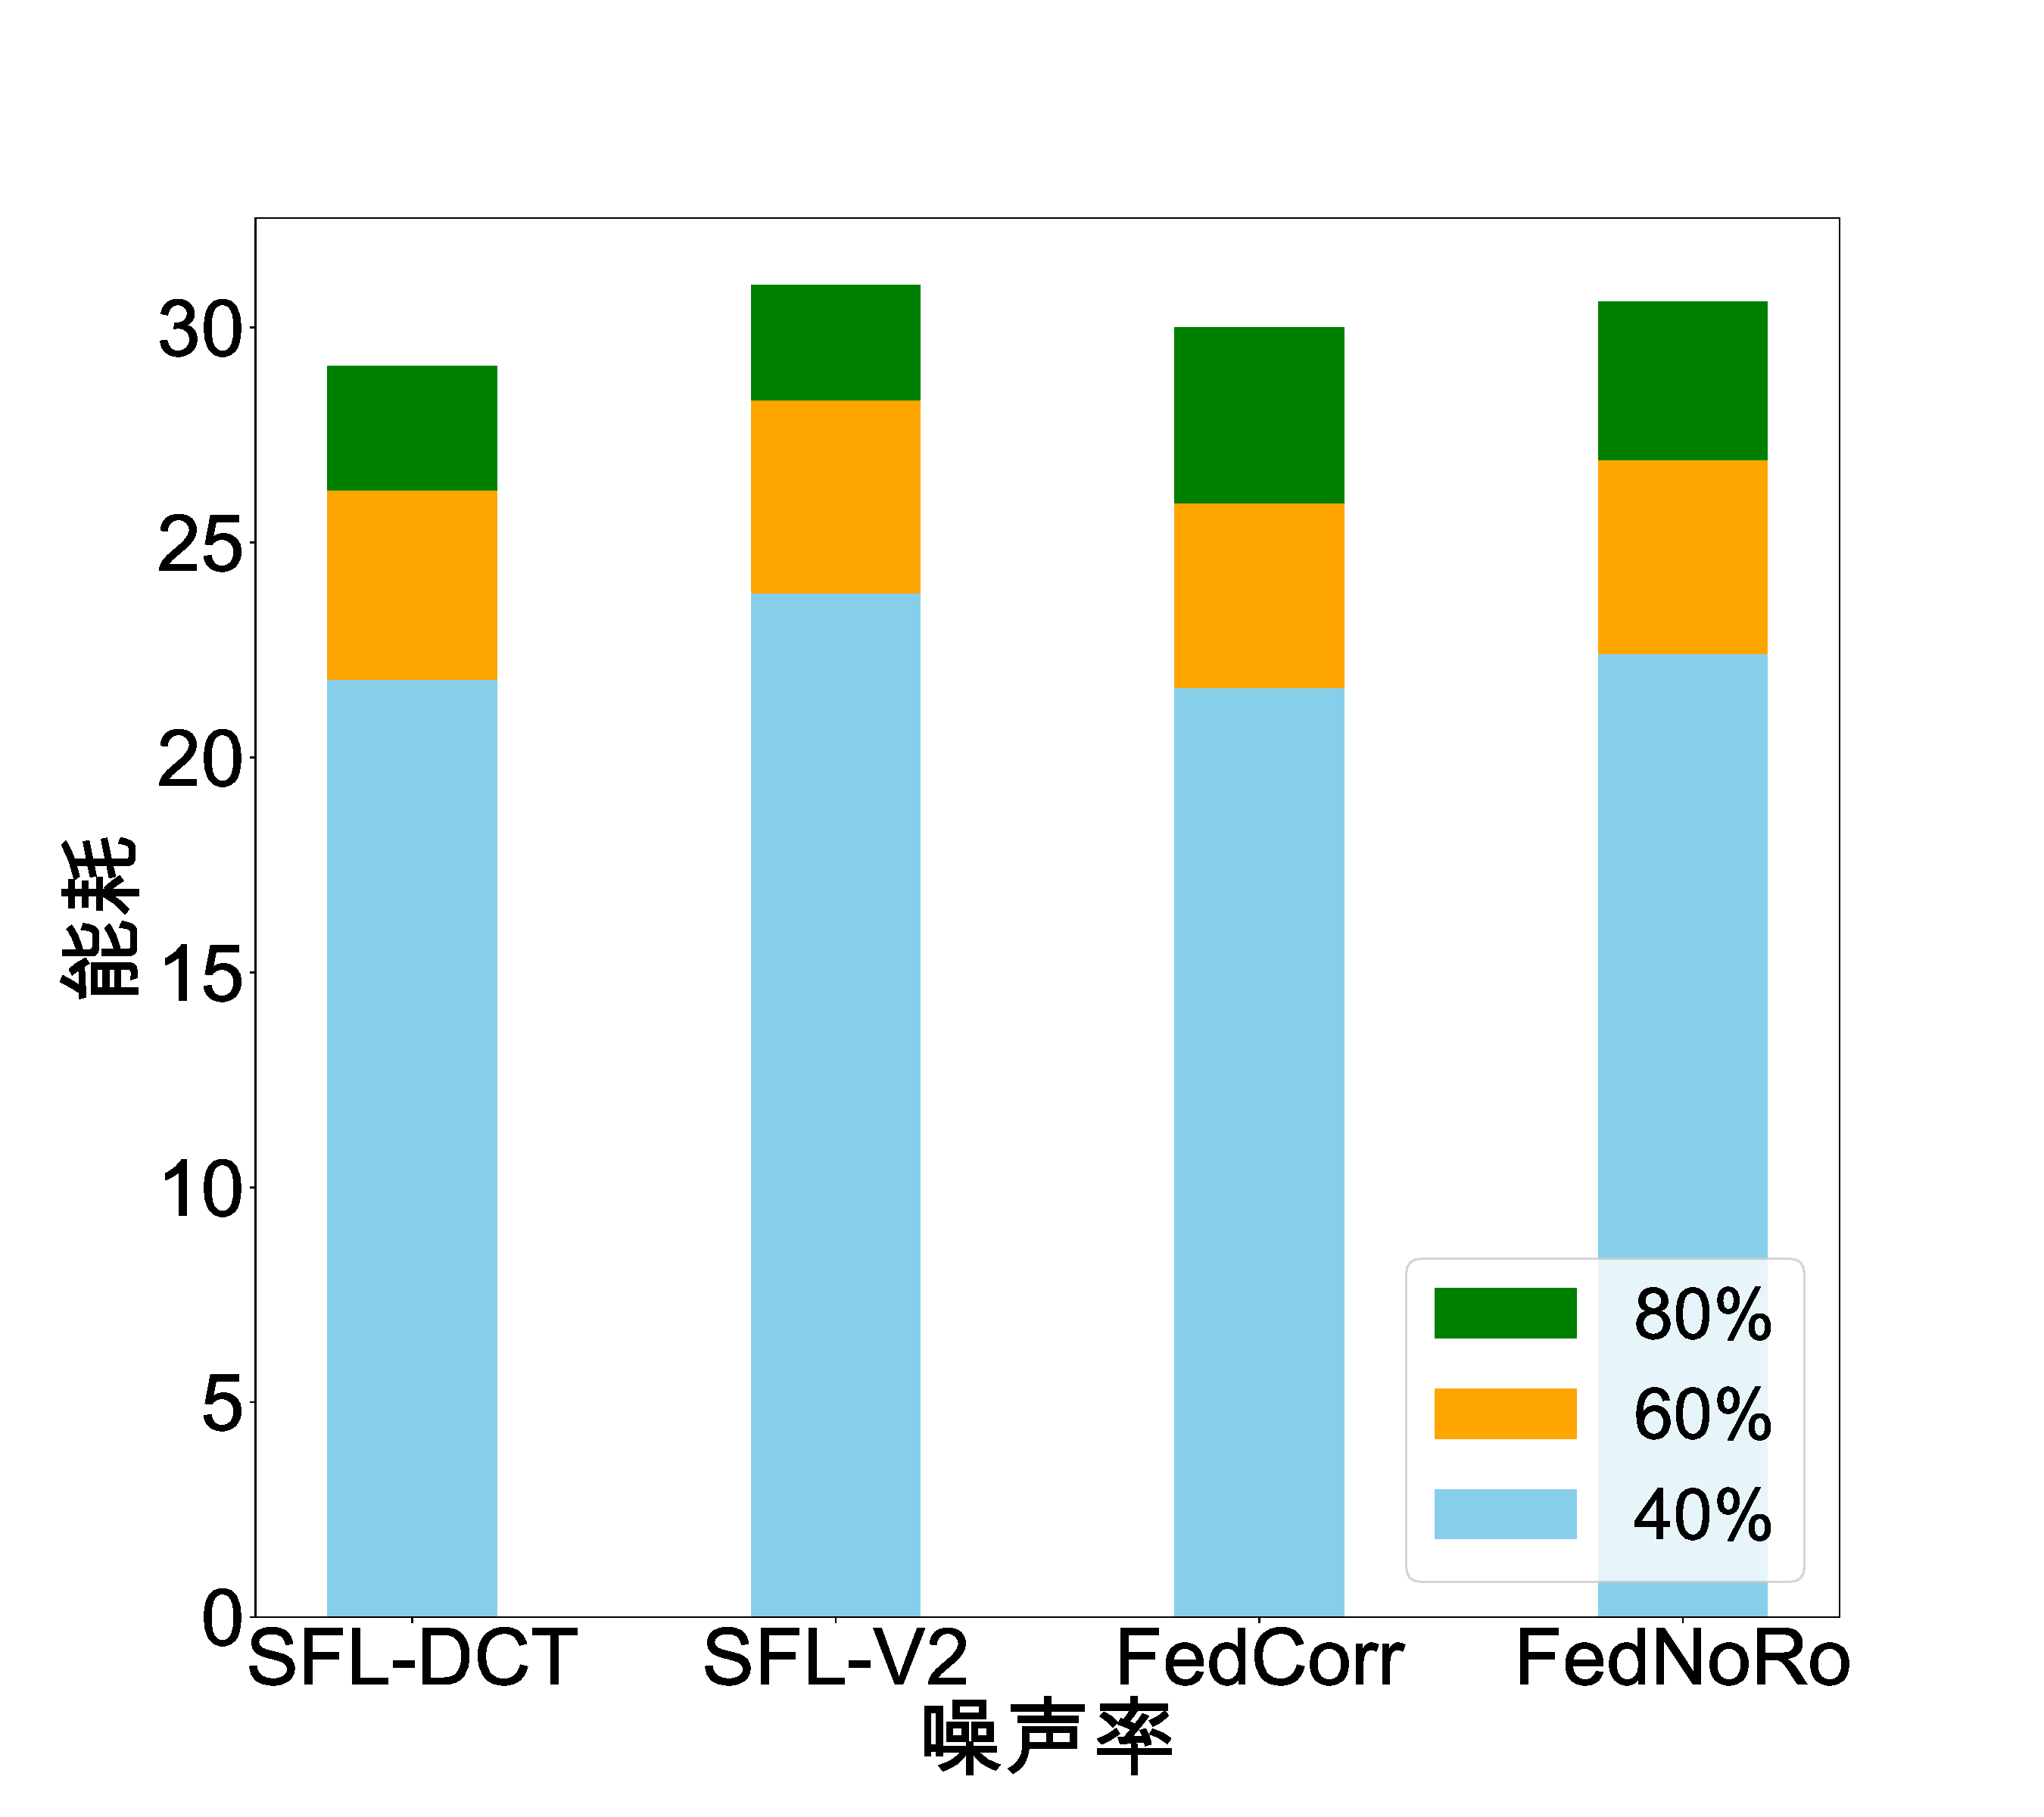
\includegraphics[width=\linewidth]{figures/power_iid.pdf}
\caption{Fashion-MNIST(IID)}
\label{fig:mnist_iid}
\end{subfigure}
\hfill
\begin{subfigure}{0.45\linewidth}
\centering
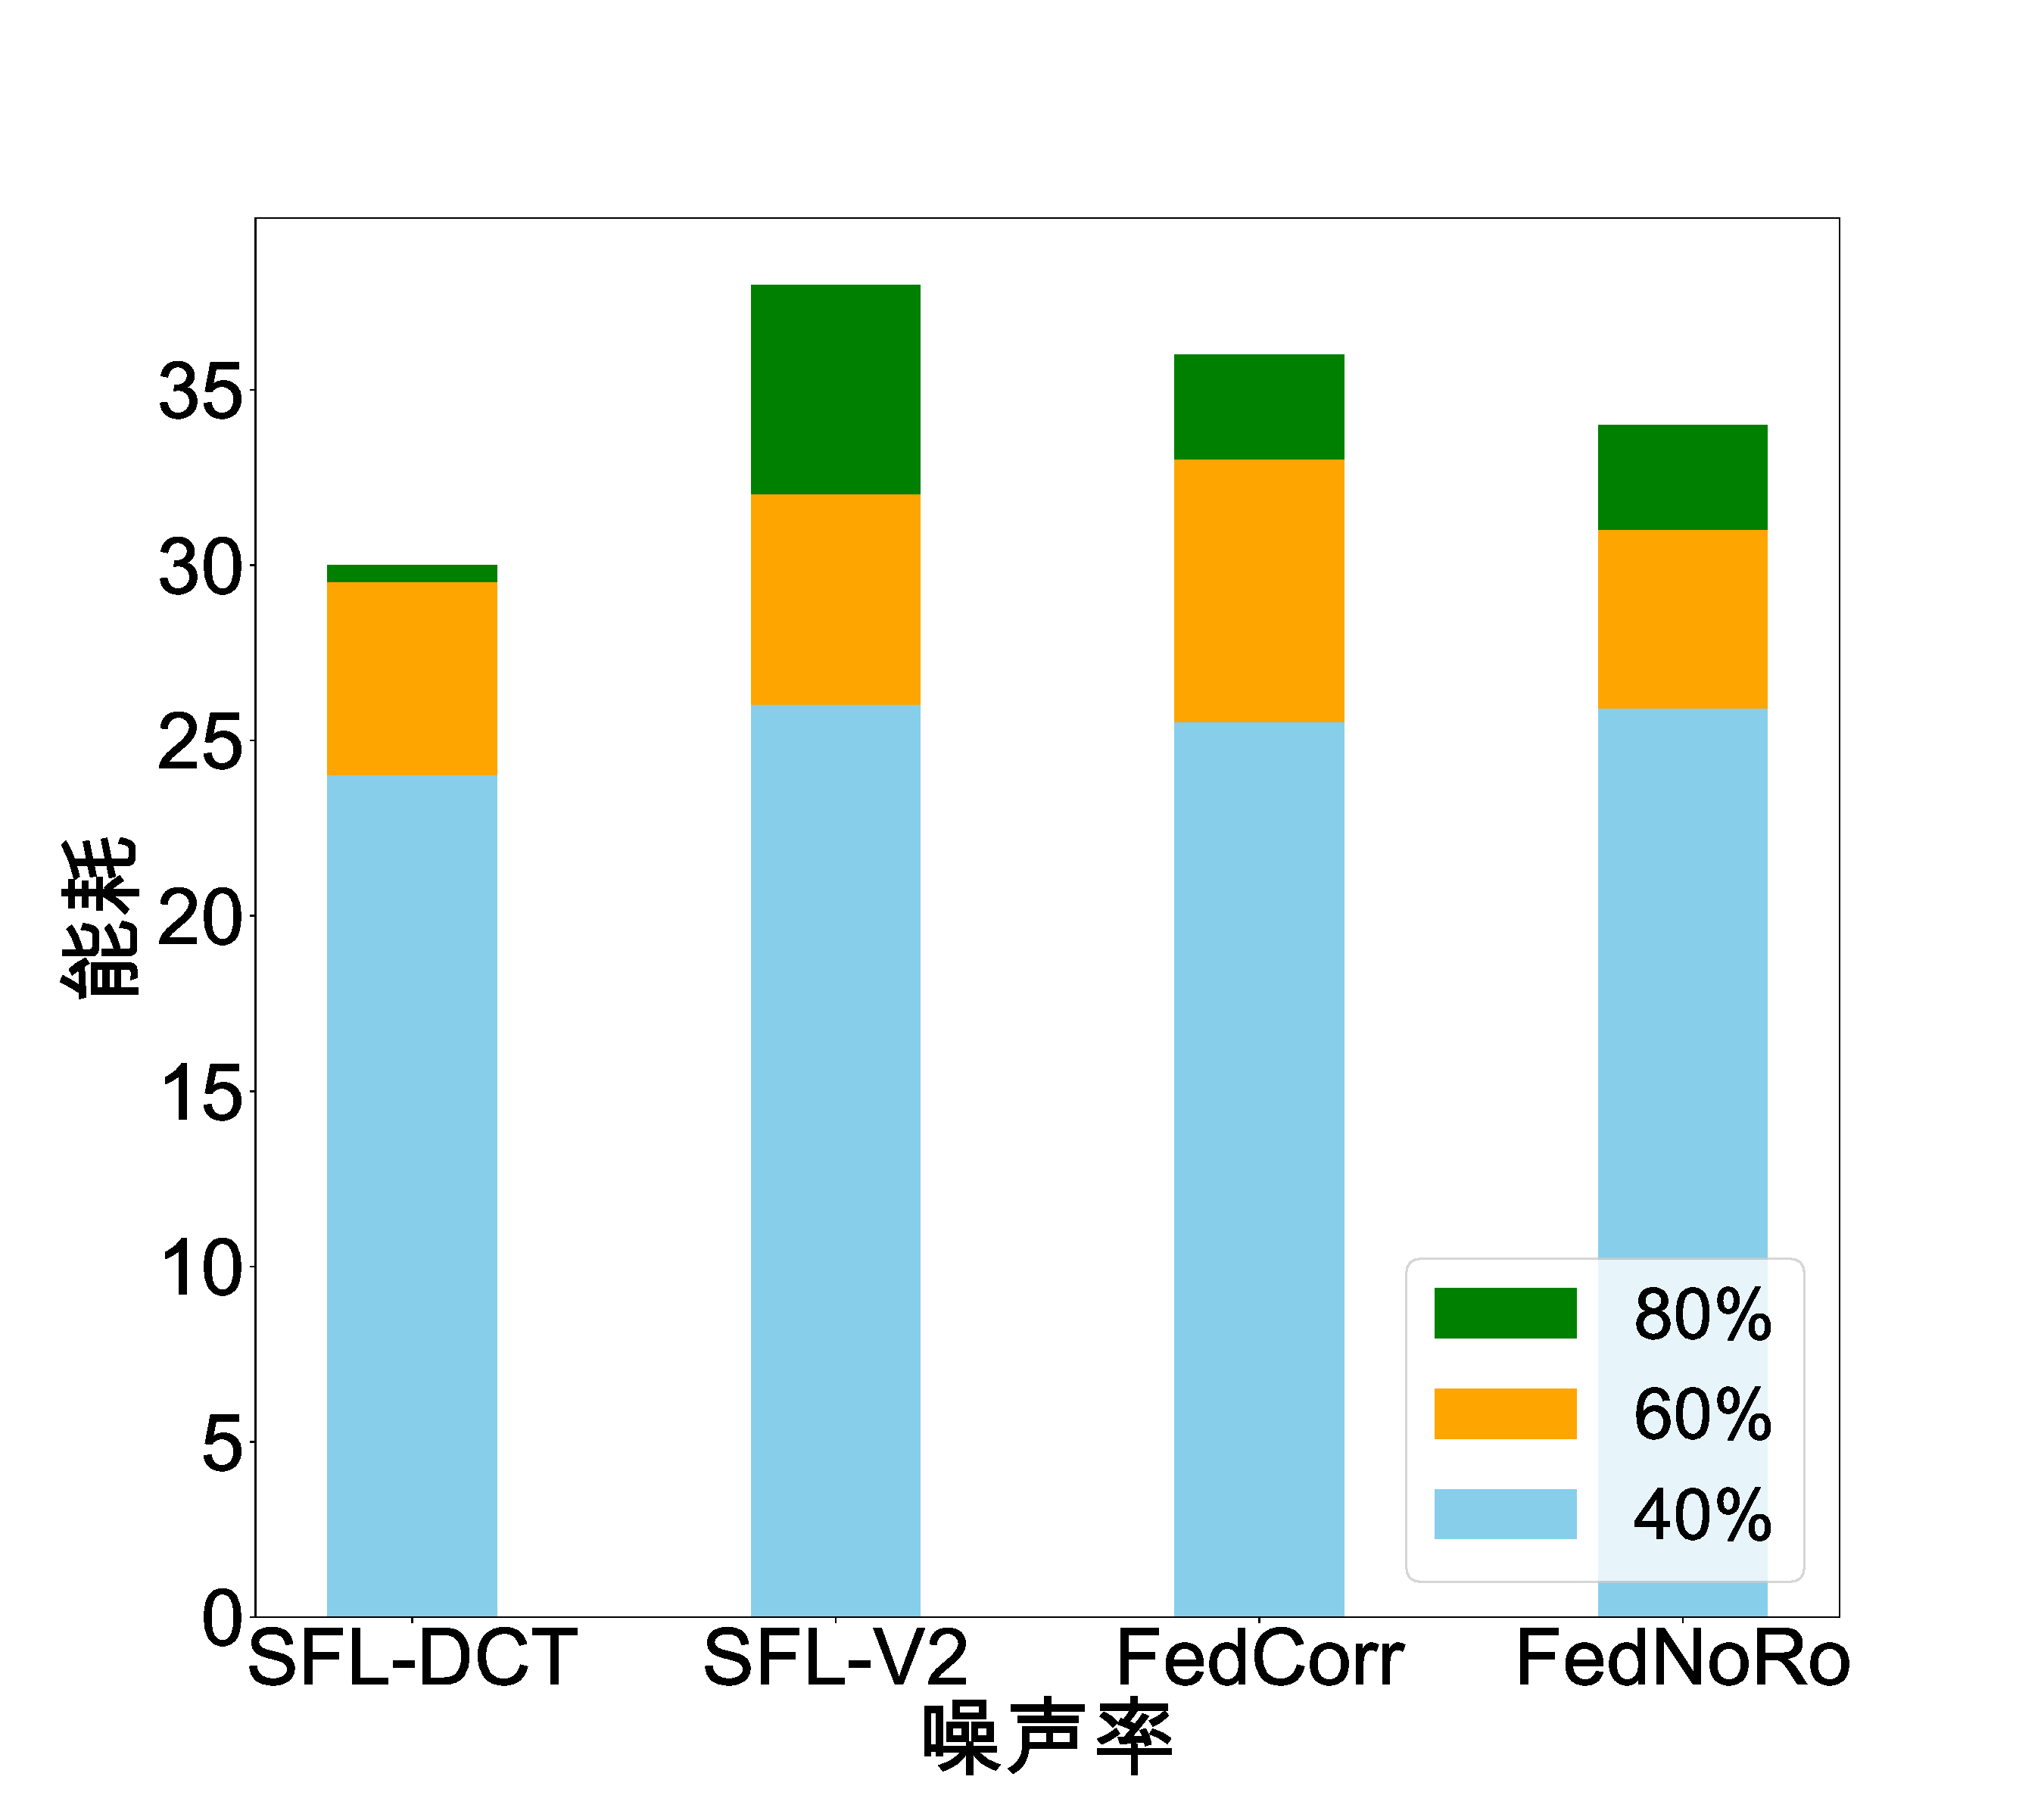
\includegraphics[width=\linewidth]{figures/power_noniid.pdf}
\caption{Fashion-MNIST(non-IID)}
\label{fig:mnist_noniid}
\end{subfigure}
\caption{不同算法的能量消耗对比。}
\label{fig:mnist_energy}
\end{figure}
我们在测试平台中进一步评估了 SF-LCT 和 SFL-V2 的真实世界收敛性和能耗（见第 \ref{sec:testbed} 节）。图 \ref{fig:testbed} 展示了我们测试平台的实验环境。本次测试使用了十个树莓派设备作为客户端，并测量了它们的总能耗。

在 SF-LCT 中，噪声标签的检测和纠正会产生额外的计算和通信开销。然而，这种开销是可量化的，并且保持最小。在树莓派测试平台上，使用 10 层 CNN 在 Fashion-MNIST 上，标准训练轮次（包括一次本地前向/反向传播和模型更新传输）平均耗时 3426 秒。SF-LCT 引入的开销分解如下：

\noindent 1) \textbf{噪声检测}：

\noindent GMM 的复杂度为 $O(|\D_n| K)$，在本实验中，GMM 每轮消耗的总时间为 1.1 秒。接下来，我们分析 LID/LE 的时间消耗。

\begin{itemize}
    \item 使用 LID 时，时间复杂度为 $O(|\D_n|^2 K)$，这是由于需要计算特征空间中数据点之间的成对距离。在本实验中，LID 每轮耗时 32.2 秒。
    \item 使用 LE 时，复杂度降低至 $O(|\D_n| K)$，因为它只需要对模型输出进行熵计算。这每轮仅耗时 0.6 秒，几乎可以忽略不计。
\end{itemize}
2) \textbf{标签纠正}：
此步骤执行一次额外的前向传播以生成高不确定性样本的软标签，时间复杂度与标准前向传播相当，即 $O(|\D_n| |\omegab|)$（$h$：隐藏层维度）。在 SF-LCT 的完整训练过程中，标签纠正总共增加了 1167 秒。

因此，SF-LCT 的额外开销为 1168.7 秒（基于 LE）至 1200.3 秒（基于 LID，$R_0=3$），与基线的完整训练过程相比，仅代表 1.13\%–1.17\% 的额外能耗。通信引起的开销已包含在上述计算中。

在每种设置下，我们测量客户端的能耗（单位：kWh），直到每个框架的模型准确率达到 SFL-V2 的收敛准确率，以便进行公平比较，因为不同框架的收敛准确率不同。图~\ref{mnist energy} 显示，SF-LCT 在达到相同收敛准确率的同时，相较于 SFL-V2 最多减少了 26.70\% 的树莓派总能耗，相较于 FedCorr 最多减少了 19.98\%，相较于 FedNoRo 最多减少了 13.31\%，相较于 FedFixer 最多减少了 14.68\%。这进一步表明，噪声检测和标签纠正过程中产生的适度资源开销是完全合理的，因为由此带来的训练效率提升是显著的。